%\documentclass[12pt]{article}
\documentclass[a4paper]{article}
\usepackage{amsmath,amsfonts,amssymb}
\usepackage[utf8]{inputenc}
\usepackage{graphicx}
\usepackage{verbatim}
\usepackage{float}
\usepackage[makeroom]{cancel} %
\usepackage[english]{babel}
\usepackage{textcomp}
\usepackage{gensymb} %
\usepackage{color}
\usepackage{subcaption}
\usepackage{caption}
%\usepackage{hyperref}
%\usepackage{physics}
%\usepackage{dsfont}
%\usepackage{amsfonts}
\usepackage{listings}
\usepackage{multicol}
\usepackage{units}
\usepackage{bm}

% From Eirik's .tex
\usepackage{epstopdf}
\usepackage{cite}
\usepackage{braket}
\usepackage{url}
\bibliographystyle{unsrt}

\usepackage{algorithmicx}
\usepackage{algorithm}% http://ctan.org/pkg/algorithms
\usepackage{algpseudocode}% http://ctan.org/pkg/algorithmicx

\usepackage[margin=1cm]{caption}
\usepackage[outer=1.2in,inner=1.2in]{geometry}

% Finding overfull \hbox
\overfullrule=2cm

\lstset{language=IDL}
 %\lstset{alsolanguage=c++}
\lstset{basicstyle=\ttfamily\small}
 %\lstset{backgroundcolor=\color{white}}
\lstset{frame=single}
\lstset{stringstyle=\ttfamily}
\lstset{keywordstyle=\color{red}\bfseries}
\lstset{commentstyle=\itshape\color{blue}}
\lstset{showspaces=false}
\lstset{showstringspaces=false}
\lstset{showtabs=false}
\lstset{breaklines}
\lstset{aboveskip=20pt,belowskip=20pt}

\lstset{basicstyle=\footnotesize, basewidth=0.5em}
\lstdefinestyle{cl}{frame=none,basicstyle=\ttfamily\small}
\lstdefinestyle{pr}{frame=single,basicstyle=\ttfamily\small}
\lstdefinestyle{prt}{frame=none,basicstyle=\ttfamily\small}
% \lstinputlisting[language=Python]{filename}


\definecolor{codepurple}{rgb}{0.58,0,0.82}
\definecolor{backcolour}{rgb}{0.95,0.95,0.92}
\definecolor{dkgreen}{rgb}{0,0.6,0}
\definecolor{gray}{rgb}{0.5,0.5,0.5}
\definecolor{magenta}{rgb}{0.58,0,0.82}

\lstdefinestyle{pystyle}{
  language=Python,
  aboveskip=3mm,
  belowskip=3mm,
  columns=flexible,
  basicstyle={\small\ttfamily},
  backgroundcolor=\color{backcolour},
  commentstyle=\color{dkgreen},
  keywordstyle=\color{magenta},
  numberstyle=\tiny\color{gray},
  stringstyle=\color{codepurple},
  basicstyle=\footnotesize,
  breakatwhitespace=false,
  breaklines=true,
  captionpos=b,
  keepspaces=true,
  numbers=left,
  numbersep=5pt,
  showspaces=false,
  showstringspaces=false,
  showtabs=false,
  tabsize=2
}

\lstset{language=[90]Fortran,
  basicstyle=\small\ttfamily,
  keywordstyle=\color{red},
  commentstyle=\color{blue},
  stringstyle=\color{dkgreen},
  morecomment=[l]{!\ },
  numbers=left,
  numbersep=5pt
}

%%%%%%%%%%%%%%%%%%%%%%%%%%%%%%%%
% Self made macros here yaaaaaay
\newcommand\answer[1]{\underline{\underline{#1}}}
\newcommand\pd[2]{\frac{\partial #1}{\partial #2}}
\newcommand\red[1]{\textcolor{red}{\textbf{#1}}}
\newcommand\numberthis{\addtocounter{equation}{1}\tag{\theequation}}
% Usage: \numberthis \label{name}
% Referencing: \eqref{name}

% Some matrices
\newcommand\smat[1]{\big(\begin{smallmatrix}#1\end{smallmatrix}\big)}
\newcommand\ppmat[1]{\begin{pmatrix}#1\end{pmatrix}}

%%%%%%%%%%%%%%%%%%%%%%%%%%%%%%%%%
% Eirik's self made macros
\newcommand{\s}{^{*}}
\newcommand{\V}[1]{\mathbf{#1}}
\newcommand{\husk}[1]{\color{red} #1 \color{black}}
\newcommand{\E}[1]{\cdot 10^{#1}}
\newcommand{\e}[1]{\ \text{#1}}
\newcommand{\tom}[1]{\big( #1 \big)}
\newcommand{\Tom}[1]{\Big( #1 \Big)}
\newcommand{\tomH}[1]{\big[ #1 \big] }
\newcommand{\TomH}[1]{\Big[ #1 \Big]}
\newcommand{\tomK}[1]{ \{ #1 \} }
\newcommand{\TomK}[1]{\Big\lbrace #1 \Big\rbrace}
\newcommand{\bigabs}[1]{\left| #1 \right|}

% Practical macros for FYS-STK4155
\newcommand{\XX}{\mathbf{X}}
\newcommand{\II}{\textbf{I}}
\newcommand{\T}{\mathsf{T}}

\newcommand{\Ey}{\mathbb{E}[\bm{\tilde y}]}
\newcommand{\xx}{\mathbf{x}}
\newcommand{\ee}{\bm{\epsilon}}
\newcommand{\yy}{\bm{\tilde y}}
\newcommand{\pr}{\text{Pr}}
\newcommand{\Nepochs}{N_{\text{epochs}}}
\newcommand{\Nbs}{N_{\text{bs}}}
\newcommand{\Nhn}{N_{h,\text{nodes}}}
\newcommand{\Nhl}{N_{h,\text{layers}}}


% Section labeling
%\usepackage{titlesec}% http://ctan.org/pkg/titlesec
%\renewcommand{\thesubsection}{\arabic{subsection}}

% Title/name/date
\title{FYS-STK4155: Project 2}
\author{Simen Nyhus Bastnes}
\date{13. November 2020}

\begin{document}
\maketitle
%%%%%%%%%%%%%%%%%%%%%%%%%%%%%%%%%%%%%%%%%%%%%%%%%
\begin{abstract}
In this project, we want to study a few methods commonly used in data science for both normal regression problems, as well as classification problems. The methods we will be employing are the stochastic gradient descent (SGD) and feed-forward neural networks (FFNN). For regression, we will be looking at is the Franke function studied in the previous project \cite{Github1}, comparing our results to the ones found there. For classification the MNIST database of handwritten digits will be studied. Cross-validation will be used for the hyperparameter search for both problems in order to make sure the model is the optimal one.
%
For the Franke function, we found that both SGD and FFNN performed worse than both OLS and Ridge, however their $R^2$ scores, $0.84$ and $0.93$ respectively, indicate that the results are not too terrible, at least not for the neural network.
%
For the MNIST data set, both the SGD and FFNN performed very well, with an accuracy of $\sim 95$\%, surpassing the results gotten with Scikit-Learn. The FFNN results are a bit weird as it seems to converge extremely fast, with very few nodes in the network.

\end{abstract}
%%%%%%%%%%%%%%%%%%%%%%%%%%%%%%%%%%%%%%%%%%%%%%%%%%%%%%%%%%%%%%%%%%%%%%%%%%%%%%%%%%%%%%%%%%
%%%%%%%%%%%%%%%%%%%%%%%%%%%%%%%%%%%%%%%%%%%%%%%%%%%%%%%%%%%%%%%%%%%%%%%%%%%%%%%%%%%%%%%%%%
\section{Introduction}
In the last two decades, computation power and availability of said machines has increased drastically, making it possible to employ more and more complex methods of solving both regression and classification problems.
\\\\
In this project, we will be looking at two different methods of performing regression and classification, and see how they compare against each other. For regression, we can also compare to the results we found in Project 1 \cite{Github1}. The methods we will be looking at is the stochastic gradient descent and a feed-forward neural network. These methods contain a few hyperparameters that will need to be adjusted in order to find the best model. In order to remove some dependency on the exact training/test data split, we will employ $k$-fold cross-validation during the hyperparameter search.
\\\\
The data sets we will be looking at is the Franke function from \cite{Franke}, as well as a reduced MNIST data set \cite{MNIST} consisting of approximately 1800 handwritten digits.
First, in Chapter \ref{chap:theory} we will briefly introduce the theory of logistic regression, and then go more in depth on stochastic gradient descent and artificial neural networks. A more in-depth description of the data sets can be found in Chapter \ref{chap:data_sets}. Then, in Chapter \ref{chap:results} we go through the results of both the Franke function and the MNIST data set, while discussing them.
Finally, we conclude our findings in Chapter \ref{chap:conclusion}.


%%%%%%%%%%%%%%%%%%%%%%%%%%%%%%%%%%%%%%%%%%%%%%%%%%%%%%%%%%%%%%%%%%%%%%%%%%%%%%%%%%%%%%%%%%
%%%%%%%%%%%%%%%%%%%%%%%%%%%%%%%%%%%%%%%%%%%%%%%%%%%%%%%%%%%%%%%%%%%%%%%%%%%%%%%%%%%%%%%%%%
\section{Theory} \label{chap:theory}
%\red{Logistic regression with softmax check aurelion geron page 195ish}
%For the derivation of the OLS method, Ridge, and Lasso regression, we will follow Chapter 2.3 and 3.4 of Hastie et al. \cite{Hastie}
\subsection{Logistic regression} \label{sec:logreg}
%In project 1, we discussed how linear regression works, and employed it to
Like with linear regression, our model is the matrix equation $\XX\beta + \bm{\epsilon}$, with $\XX$ being the design matrix consisting of $n$ inputs and $p$ predictors. The regression parameters $\beta$ is a matrix $n_{\text{classes}}$, $p$ for a classification problem with $K$ categories/classes. We want the output to be the probability that the input belongs to a specific class. From \cite{Hastie} Eq 4.18, we get that the probabilities are.
\begin{align*}
	\pr(G = k | X = x) &= \frac{\exp(\beta_{k0}+\beta{k}^\T x)}{1 + \sum_{l=1}^{K-1}\exp(\beta_{l0} + \beta_l^\T x)}, \,\text{for}\,k=1, \dots, K-1\\
	\pr(G = K | X = x) &= \frac{1}{1 + \sum_{l=1}^{K-1}\exp(\beta_{l0} + \beta_l^\T x)}
%	\log(\frac{\Pr(G=1|X=x)}{\Pr(G=K|X=x)} &= \beta_{10} + \beta_1^\T x\\
%	\log(\frac{\Pr(G=2|X=x)}{\Pr(G=K|X=x)} &= \beta_{20} + \beta_2^\T x\\
%	&\vdots\\
%	\log(\frac{\pr(G=K-1|X=x)}{\Pr(G=K|X=x)} &= \beta_{(K-1)0} + \beta_{K-1}^\T x\\
\end{align*}
And the probabilities sum to one. To classify a sample, we take $\operatorname{argmax}(Pr)$. To fit this, we use the maximum likelihood, and want to maximize the probability of seeing the observed data. The log-likelihood for $N$ observations is given by
\begin{align*}
 \ell(\theta) &= \sum_{i=1}^N\log p_{g_i}(x_i;\theta)
\end{align*}
where $p_k(x_i;\theta) = \Pr(G=k|X=x_i;\theta)$. The cost/loss function is the negative log-likelihood. Following \cite{Geron} we get the cost-function for the so-called cross-entropy for $N$ observations and $K$ classes
\begin{align*}
	C(\beta) = -\frac{1}{N}\sum_{i=1}^N\sum_{k=1}^K y_k^{(i)}\log(p_k^{(i)})
\end{align*}
where $y_k^{(i)}$ is a one-hot vector (equal to 1 if the class is k, 0 otherwise). As with linear regression we can add additional regularization terms like we did with Ridge and Lasso regression. The question now is how to find the optimal regression coefficients $\beta$, and one of these methods is the gradient descent method.
\subsection{Stochastic gradient descent} \label{sec:sgd}
Gradient descent is an optimization algorithm that finds local minimums by computing the gradient for the loss function with regards to the current coefficients $\beta$ (or weights when dealing with neural networks). Since the gradient points in the direction of the fastest ascent, the negative gradient points in the direction where the loss function decreases the most. Then, we take a step towards the local minimum by subtracting the coefficients with some factor multiplied with the gradient w.r.t. that coefficient. This is the learning rate, and picking the correct value for this learning rate is critical in how fast the GD converges. Too large, and the solution won't converge. If the loss function is convex, the local minimum is also the global minimum. The starting point $\beta^{(0)}$ is usually set to random normal distributed values.
\\\\
Algorithm \ref{alg:gd} shows the normal gradient descent method, where $\eta$ is the learning rate (where we do a set amount of steps/epochs, but we could have just continued until the gradient reaches zero, or below some threshold)
\begin{algorithm}[H]
\caption{Gradient descent}
\begin{algorithmic}[1]
\State Given $\XX$, $y$, $\beta^{(0)}$, $\eta$
\For{$i = 0$, $N_{\text{epochs}}-1$}
\State Compute $\nabla_i$ from $\beta^{(i)}$
\State (Update learning rate $\eta$ if not using constant learning rate)
\State $\beta^{(i+1)} = \beta^{(i)} - \eta \nabla_i$
\EndFor
\end{algorithmic}
\label{alg:gd}
\end{algorithm}
One of the problems with the gradient descent is that it is extremely computationally heavy to compute the full gradient at every step, especially for a large set of inputs and parameters. Another problem is that you end up at a local minimum, so results are very dependent on the starting values. One of the ways to reduce these problems is the stochastic gradient descent, where instead of computing the full gradient, for each step, a single random instance of the training set is chosen, and the gradient descent step is done based only on that instance. Thus, each step is significantly faster, but each step won't take the direction of the fastest descent due to the random nature. However this also means that the algorithm can jump out of local minima, making it more likely to find the global minimum. In this project specifically, we will be implementing the minibatch stochastic gradient descent, where we compute a random mini-batch for each step instead of just one instance. Algorithm \ref{alg:sgd} shows the minibatch SGD.
\begin{algorithm}[H]
\caption{Stochastic Gradient descent}
\begin{algorithmic}[1]
%\State Given $\XX$, $y$, $\beta^{(0)}$, $\eta$
\For{$i = 0$, $N_{\text{epochs}}-1$}
\State Shuffle $\XX_{\text{train}}$ and $y_{\text{train}}$
\State Split into $N_{\text{mb}}$ minibatches
\For{$j=0$, $N_{\text{mb}}$}
\State Compute gradient using minibatch $j$
\State Update $\beta$
\EndFor
%\State (Update learning rate $\eta$ if not using constant learning rate)
%\State $\beta^{(i+1)} = \beta^{(i)} - \eta \nabla_i$
\EndFor
\end{algorithmic}
\label{alg:sgd}
\end{algorithm}
One of the ways we can assure that the SGD stops at a reasonable point is to scale the learning rate with the number of steps taken. This way, the first steps we do are the largest, and allows the algorithm to jump around the different minima, and as we continue, the step size is decreased and we try to go towards the minimum we are currently in. How the learning rate changes over time is often called the learning schedule, and the way we will be testing in this project is as follows.
\begin{align*}
	\eta_t &= \frac{t_0}{t + t_1}
\end{align*}
where $t_0$ and $t_1$ are parameters we have to tune, and $t = i\cdot N_{\text{mb}} + j$ (following the notation from Algorithm \ref{alg:sgd})
\\\\
For our regression problem, with a mean squared error loss function, the gradient can be expressed as
\begin{align*}
	\nabla_{\beta}C(\beta) = \frac{2}{n}X^\T(X\beta-y)
\end{align*}
And for multiclass logistic regression with cross-entropy as our loss function, the gradient is given by
\begin{align*}
	\nabla_{\beta}C(\beta) = X^\T(p-y)
\end{align*}
Ridge regularization ($L^2$ norm) can be added to the gradients by simply adding a term $\lambda \cdot \beta$.
\subsection{Artificial neural networks}
The concept behind an artificial neural network (ANN) is a system that attempts to simulate the behavior of neurons in a human mind. While the idea was introduced as early as 1943 \cite{mcculloch43a}, its use has only really exploded in recent years thanks to the processing power available. The type of neural net we are looking at here is the so-called feed-forward neural net, which consists of a number of "neurons" or "nodes" structured in several layers, where each node in one layer is connected to all the nodes in the next layer. This net has at least three layers; one input layer, one output layer, and at least one hidden layer. From the universal approximation theorem, a neural net with at least one hidden layer can be used to approximate "all" types of functions. The amount of neurons in each layer and the amount of hidden layers is up to the user, and determining which sets of parameters approximates the problem best can be difficult.
\\\\
Information is fed through forward through the system, going from layer to layer until it reaches the output layer. Each connection between nodes have a weight associated with them, giving us that the input in the first hidden layer is given by the matrix equation
\begin{align*}
	z_i &= \mathbf{w_i}^T \mathbf{x} + b_i
\end{align*}
where $\mathbf{x}$ is the input, $\mathbf{w}$ is the weights connecting the node in the hidden layer with all the nodes in the input layer, and $b_i$ is the bias term for each node. This is then fed through an activation function $\sigma(z)$ which determines whether or not that node "fires" based on the input, giving us that the output from a node is given by
\begin{align*}
	a_i &= \sigma(z_i) 
\end{align*}
Examples of the activation functions used is shown in Section \ref{sec:act_fun}, and is also an important part in trying to figure out which model fits best. Each layer can have different activation functions. Once all the outputs $a$ for a layer is computed, we continue to the next layer all the way until the end. This is called the forward pass, and the output is the neural nets prediction given the input.
\subsection{Back-propagation}\label{sec:backprop}
Since the first prediction is probably pretty bad, we need to adjust the weights. This is done via gradient descent, in a process called back-propagation. Using the loss function, we compute the gradient, and go backwards through the neural net to update the weights and bias. Then, the process is repeated based on the new prediction.
\\\\
Following \cite{Nielsen}, the first step in the back-propagation is to compute the error in the output layer
\begin{align*}
	\delta^L &= \nabla_a C\odot\sigma'(z^L)
\end{align*}
we see that it depends on the derivative of both the loss function and the output layer activation function. The exact expressions for our cases is given in Section \ref{sec:loss}. Then we compute the error recursively for the previous layers
\begin{align*}
\delta^l = ((w^{l+1})^T \delta^{l+1}) \odot \sigma'(z^l)
\end{align*}
Then we have the following equations for the gradient w.r.t. the bias and weights
\begin{align*}
	\frac{\partial C}{\partial w^l_{jk}} &= a^{l-1}_k \delta^l_j\\
	\frac{\partial C}{\partial b^l_j} &= \delta^l_j
\end{align*}
Which we can use to update the weights and bias like we discussed earlier for gradient descent.
\subsection{Activation functions}\label{sec:act_fun}
In order to do the forward pass and back-propagation, we need expressions for both the activation function $\sigma(z)$ and their derivative. Some of the most common activation are listed below.\\
First, we have the sigmoid function
\begin{align*}
	\sigma(z) &= \frac{1}{1+\exp(z)}
\end{align*}
and its derivative
\begin{align*}
	\sigma'(z) &= \sigma(z)(1-\sigma(z))
\end{align*}
ReLU (Rectified Linear Unit)
\begin{align*}
    \sigma(z) = 
    \begin{cases}
        z & \text{if } z \geq 0 \\
        0 & \text{if } z < 0 \\
    \end{cases}
\end{align*}
and its derivative
\begin{align*}
    \sigma(z) = 
    \begin{cases}
        1 & \text{if } z \geq 0 \\
        0 & \text{if } z < 0 \\
    \end{cases}
\end{align*}
Leaky ReLU
\begin{align*}
    \sigma(z) = 
    \begin{cases}
        z & \text{if } z \geq 0 \\
        0.01z & \text{if } z < 0 \\
    \end{cases}
\end{align*}
and its derivative
\begin{align*}
    \sigma(z) = 
    \begin{cases}
        1 & \text{if } z \geq 0 \\
        0.01 & \text{if } z < 0 \\
    \end{cases}
\end{align*}
Hyperbolic tangent
\begin{align*}
	\sigma(z) &= \tanh(z)
\end{align*}
and its derivative
\begin{align*}
	\sigma'(z) &= 1-\tanh(z)^2
\end{align*}
For our output layers we will be using the following activation functions. For regression, the activation function is just identity.
\begin{align*}
	\sigma(z) &= z\\
	\sigma'(z) &= 1
\end{align*}
And for classification we use the softmax function
\begin{align*}
	\sigma(z_i) &= \frac{\exp(z_i)}{\sum_k\exp(z_k)}\\
	\sigma'(z_i) &= z_i(\delta_{ij} - z_j)
\end{align*}
where $\delta_{ij}$ is the Kronecker delta.
\subsection{Loss functions and their gradient} \label{sec:loss}
Since the error of the output layer depends on both the gradient of the loss function as well as the derivative of the output activation function, we want to look at what that expression is for our cases. First, for regression, we use the mean squared error as our loss function. For a single sample, this is
\begin{align*}
C_{\text{MSE}} = \frac{1}{2}(a^L - y)^2
\end{align*}
the derivative with respect to $a$ is then
\begin{align*}
\pd{C_{\text{MSE}}}{a^L} &= a^L - y
\end{align*}
With the identity function as the output activation function, this gives us that the error in the output layer is
\begin{align*}
	\delta^L &= \nabla_a C\odot\sigma'(z^L) = a^L - y
\end{align*}
For the classification problem, we use the softmax function as the output activation function, and Cross-Entropy for the loss function.
\begin{align*}
C_{\text{CE}} &= -\sum_{i=1}y_i\log a^L
\end{align*}
The output error can be shown to be
\begin{align*}
	\delta^L &= a^L - y
\end{align*}
which is very nice and the same as we found for the regression case. With other combinations of activation and loss functions this will probably not be as well behaved.
\subsection{Learning rate and weight initialization} \label{sec:weights}
For the learning rate, we will be looking at the two same methods as described earlier in Section \ref{sec:sgd}, where we either keep it constant, or scale it with the number of iterations.
\\\\
In order to start the training of the neural network, we need to set some starting value for the weights and bias. One way to do this is to set the weights to random normal distributed values. The bias is set to some small value in order to avoid problems with vanishing gradients.
\\\\
Another method of initializing the weights and bias is the way described in \cite{glorot}, where the weights and bias is drawn from a uniform distribution between
\begin{align*}
	\bigg[-\frac{\sqrt{6}}{\sqrt{n_j + n_{j+1}}}\,, \frac{\sqrt{6}}{\sqrt{n_j + n_{j+1}}}\bigg]
\end{align*}
where $n_j$ is the amount of nodes in the previous layer, and $n_{j+1}$ is the amount of nodes in the current layer.

\subsection{Measure of performance} \label{sec:performance}
In order to gauge how good our model functions, we will be looking at the mean squared error and $R^2$ score for the regression problems. The equations for those can be found in \cite{Github1}. For the classification case, we are interested in the accuracy score, which is the number of correctly guessed targets $t_i$ divided by the total number of targets.
\begin{align*}
	\text{Accuracy} &= \frac{\sum_{i=1}^n I(t_i = y_i)}{n}
\end{align*}
where $I$ is the indicator function, which is 1 if $t_i = y_1$ and 0 otherwise. $y_i$ is the output from the forward pass.
%%%%%%%%%%%%%%%%%%%%%%%%%%%%%%%%%%%%%%%%%%%%%%%%%%%%%%%%%%%%%%%%%%%%%%%%%%%%%%%%%%%%%%%%%%
%%%%%%%%%%%%%%%%%%%%%%%%%%%%%%%%%%%%%%%%%%%%%%%%%%%%%%%%%%%%%%%%%%%%%%%%%%%%%%%%%%%%%%%%%%
\section{Data sets} \label{chap:data_sets}
In this project, we will be using two different data sets. The first, is the Franke function we looked at in the previous project \cite{Github1}. The equation for the Franke function can be found there and in \cite{Franke}. This function is a two-dimensional function that has been widely used for testing implementations for regression and interpolation.
\\\\
%
The second data set is the so-called MNIST data set \cite{MNIST}, which is a large data set consisting of handwritten digits from 0 to 9, and is commonly used for testing various types of classification methods. The original data set consists of 70 000 images of size $28\times28$ pixels. However, as the scope of this project is fairly limited, we will be looking at a reduced version of the data set both in size and resolution in order to have time to produce results. The specific version of the data set we will be using is the one available within the scikit-learn python package, and consists of 1797 images of size $8\times8$ pixels. Figure \ref{fig:digits} shows an example of some of the images in the data set. For the full resolution MNIST data set, human accuracy has been noted to be roughly $0.2$\%, according to \cite{c2012}. However, given the reduction in resolution, it is not unlikely that it would be somewhat lower for the data set we will be looking at.
\begin{figure}[H]
	\centering
	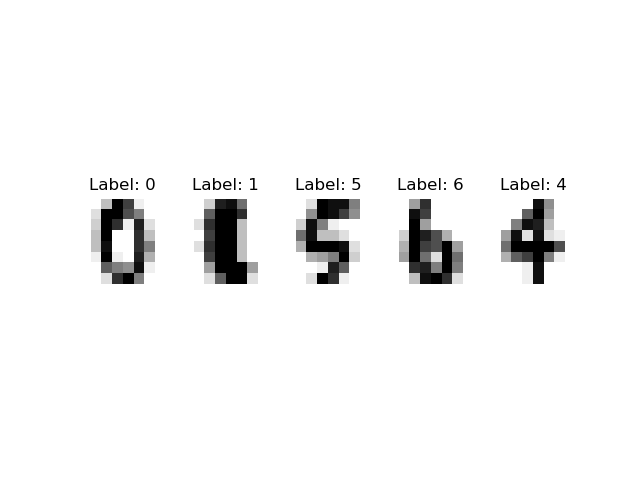
\includegraphics[scale=0.6]{../figures/digits.png}
	\caption{Some of the images in the reduced MNIST data set, with their label printed above.}
	\label{fig:digits}
\end{figure}
%\red{MNIST, show example plot of some of the 8x8 images with labels}
%The second data set is terrain elevation maps taken from \cite{terrain}, and the maps are stored in the GeoTIFF file format, and are from the SRTM Arc-Second Global data set. In the \texttt{datafiles} folder there are three maps, each of one region of Norway, though only one of them, \\\texttt{SRTM\_data\_Norway\_3.tif} is studied in this project. This map is over the south-eastern part of Norway. A plot of the entire map, as well as a more detailed description of the location is given in figure \ref{fig:entiremap} in appendix \ref{app:terrain}.
%%%%%%%%%%%%%%%%%%%%%%%%%%%%%%%%%%%%%%%%%%%%%%%%%%%%%%%%%%%%%%%%%%%%%%%%%%%%%%%%%%%%%%%%%%
%%%%%%%%%%%%%%%%%%%%%%%%%%%%%%%%%%%%%%%%%%%%%%%%%%%%%%%%%%%%%%%%%%%%%%%%%%%%%%%%%%%%%%%%%%
\section{Results and discussion} \label{chap:results}
The code used to generate the results presented in this section can be found in the Github repository \cite{Github2}. For both data sets, we employ cross-validation when searching for the hyperparameters. The results section will be split into, the first one pertaining to the Franke function, while the second contains the analysis of the MNIST data set
\\\\
For simplicity, for all the neural network results we will deal with hidden layers consisting of identical amount of nodes, using the same activation functions for all layers. Strictly speaking there is nothing stopping us from having arbitrary choices of amount of nodes for the layers in the network, and some neural net structures (like for example autoencoders) rely on that. Taking this into account drastically increases the potential things to test, and is thus outside of the scope of this report.

\subsection{Franke function}
First, we look at the results from the Franke function. As we are primarily interested in seeing how both the SGD and FFNN compares our results in \cite{Github1} where we used OLS and Ridge-regression, we will be looking at the same realization of the Franke function, with $N=529$ randomly drawn points with a noise level of $\sigma=0.05$.
\subsubsection{Stochastic Gradient Descent}
For the stochastic gradient descent results, we use the same approach to creating the design matrix $\XX$ as we did in \cite{Github1}, where each predictor is a combination of polynomial degrees of $x$ and $y$. While we could have performed the SGD for the same range of polynomial degree $p$ as we did there, due to time limitations we will focus on the values of $p$ which gave the best test error for both OLS and Ridge. This was found to be $p=8$ for OLS, and $p=15$ for Ridge. The hyperparameters we want to adjust for our stochastic gradient descent is shown in Table \ref{tab:hyper_sgd}.% shows the hyperparameters we are able to adjust for our stochastic gradient descent
\begin{table}[H]
  \centering
  \caption{Different hyperparameters for minibatch SGD.}
  \label{tab:hyper_sgd}
  \begin{tabular}{c|c}
    \hline\hline
    \textbf{Hyperparameter} & \textbf{Description}\\\hline
    $N_{\text{epochs}}$ & Number of epochs \\
    batch size & size of each minibatch \\
    $\eta_0$ & Learning rate \\
    $\lambda$ & $L^2$ regularization strength
    \end{tabular}
\end{table}
As mentioned earlier, we also want to look at a training schedule where the learning rate gets smaller with the number of iterations. Sadly, due to time constraints, we will only compare a single set of $(t_0, t_1)$ against the number of epochs, as it is the most relevant. %\red{?????????????????}
\\\\
With the learning rate set as constant, we try to fit our model with the following sets of hyperparameters, going through each combination and computing the test error for each one.
\begin{align*}
	N_{\text{epochs}} &\in \{10, 25, 50, 100\}\\
	\text{batch size} &\in \{1, 5, 10, 50\}\\
	\eta_0 &\in \{0.1, 0.01, 0.001\}\\
	\lambda &\in \{0.0, 0.1, 0.01, 0.001\}
\end{align*}
Table \ref{tab:sgd_best_fit8} shows the best-fit parameters for this data set and set of hyperparameters.
\begin{table}[H]
  \centering
  \caption{Best-fit hyperparameters for Franke function SGD, $p=8$}
  \label{tab:sgd_best_fit8}
  \begin{tabular}{c|c}
    \hline\hline
    Parameter & Value\\\hline
    $\Nepochs$ &  $100$\\
    batch size &  $5$\\
    $\eta_0$ & $0.1$ \\
    $\lambda$ & $0.0$
    \end{tabular}
\end{table}
To see how the different hyperparameters interact, we plot heatmaps with the different hyperparameters on the $x$ and $y$ axis, and either MSE or $R^2$ for the $z$ values. Since both of them should show the same trends, we opt to look at the $R^2$ score since the specific values makes it easier to determine how good the fit is.
\\\\
Figure \ref{fig:sgd_1} shows the $R^2$ score for the number of epochs plotted against the learning rate, where all the other parameters are set to the best-fit parameter shown in table \ref{tab:sgd_best_fit8}. We see that the smallest learning rate and fewest amount of epochs give the worst fit by far. As either the step size is increased or the number of epochs, the fit improves, indicating that the model manages to converge more towards a minimum.
\begin{figure}[H]
	\centering
	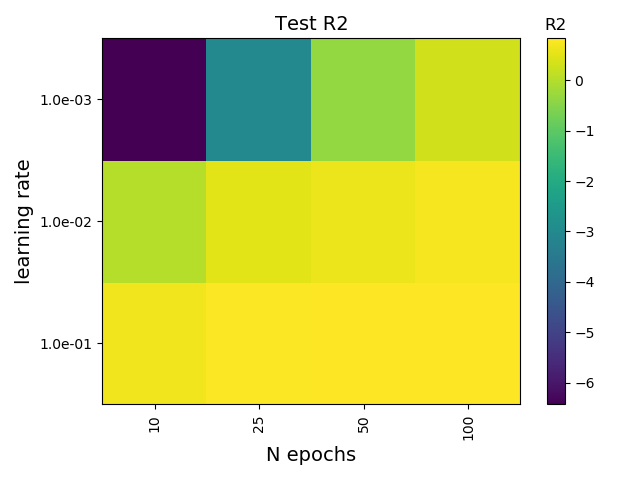
\includegraphics[scale=0.5]{../figures/task_a/test_p8/heatmap_test_p8_lr_constant_Nhyp4434_R2_n_epochs_eta0.png}
	\caption{$R^2$ score for number of epochs plotted against learning rate. All other parameters are set to the best-fit values.}
	\label{fig:sgd_1}
\end{figure}
Figure \ref{fig:sgd_2} shows $\Nepochs$ plotted against batch size. We see that most values yield decent results, though higher $\Nepochs$ and batch size greater than 1 gives the best result. For some reason, $\Nepochs=100$ and batch size $=1$ gives a really horrible result, which might indicate that the learning rate is not ideal for that specific case, or some other parameter. Since the value is the average of all the $k$-folds, it seems unlikely that it is purely due to back luck with starting values.
\begin{figure}[H]
	\centering
	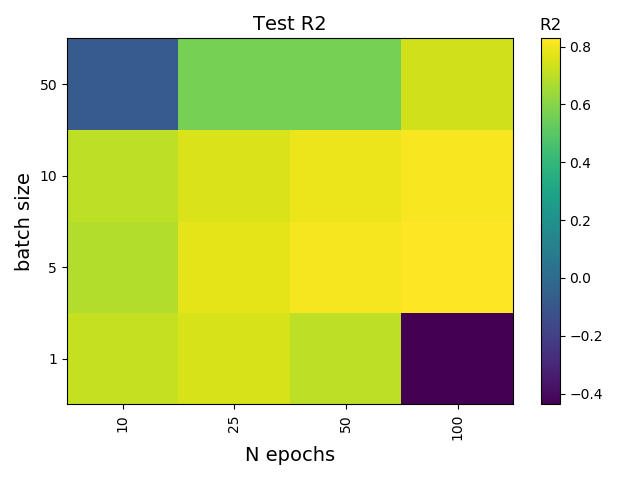
\includegraphics[scale=0.5]{../figures/task_a/test_p8/heatmap_test_p8_lr_constant_Nhyp4434_R2_n_epochs_bsize.png}
	\caption{$R^2$ score for number of epochs plotted against the batch size. All other parameters are set to the best-fit values.}
	\label{fig:sgd_2}
\end{figure}
Figure \ref{fig:sgd_3} shows the number of epochs plotted against the Ridge regularization $\lambda$. Like we saw in project 1, the model seems to prefer the lower values of $\lambda$, and the largest $\lambda = 0.1$ gives terrible results for all $\Nepochs$.
\begin{figure}[H]
	\centering
	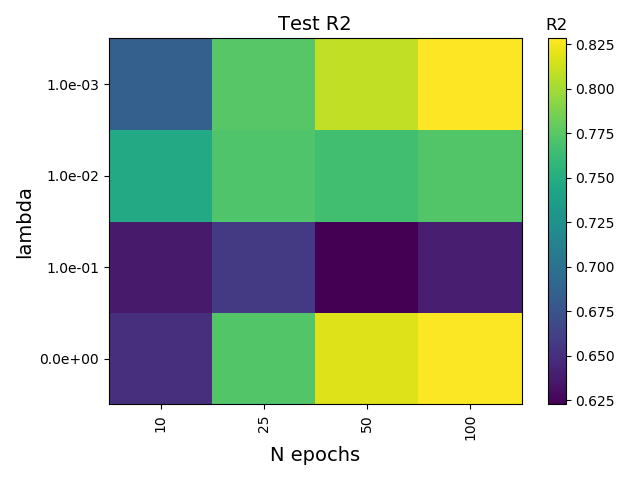
\includegraphics[scale=0.5]{../figures/task_a/test_p8/heatmap_test_p8_lr_constant_Nhyp4434_R2_n_epochs_lambdas.png}
	\caption{$R^2$ score for number of epochs plotted against regularization $\lambda$. All other parameters are set to the best-fit values.}
	\label{fig:sgd_3}
\end{figure}
Moving on to the $p=15$ case, we fit the model with the parameters, and get the following best fit, shown in Table \ref{tab:sgd_best_fit15}
\begin{table}[H]
  \centering
  \caption{Best-fit hyperparameters for Franke function SGD, $p=15$}
  \label{tab:sgd_best_fit15}
  \begin{tabular}{c|c}
    \hline\hline
    Parameter & Value\\\hline
    $\Nepochs$ &  $100$\\
    batch size &  $5$\\
    $\eta_0$ & $0.1$ \\
    $\lambda$ & $0.001$
    \end{tabular}
\end{table}
Which interestingly enough is the same as for $p=8$ except that the regularization is now $\lambda = 0.001$ instead of zero. The preferred $\lambda$ for Ridge in \cite{Github1} was $5.46\cdot10^{-6}$, however we did not test for $\lambda$ values that low.
\\\\
Figure \ref{fig:sgd_4} shows the same three heatmap plots plotted for $p=15$. The learning rate vs number of epochs is mostly identical, however the batch size plotted against $\Nepochs$ shows that something weird is happening. For some reason, the smallest batch size causes an overflow. The bottom panel, showing the regularization plotted against $\Nepochs$ is also mostly similar to the one shown in Figure \ref{fig:sgd_3}

\begin{figure}[H]
  \centering
  \begin{subfigure}{0.49\textwidth}
    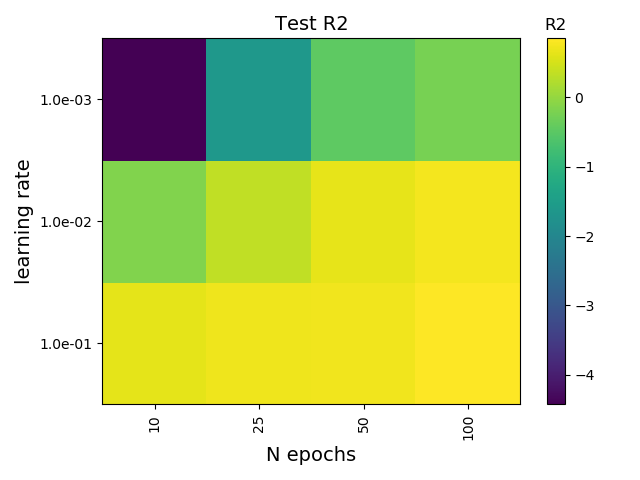
\includegraphics[scale=0.45]{../figures/task_a/test_p15/heatmap_test_p15_lr_constant_Nhyp4434_R2_n_epochs_eta0.png}
    \caption{$\Nepochs$ vs learning rate}
  \end{subfigure}
  \begin{subfigure}{0.49\textwidth}
    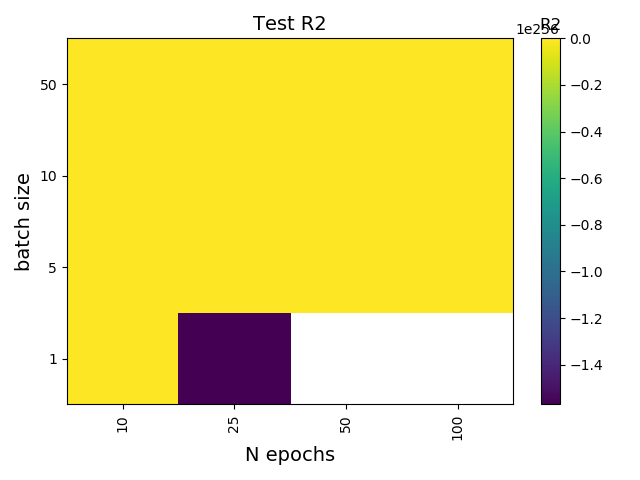
\includegraphics[scale=0.45]{../figures/task_a/test_p15/heatmap_test_p15_lr_constant_Nhyp4434_R2_n_epochs_bsize.png}
    \caption{$\Nepochs$ vs batch size}
  \end{subfigure}\\
  \begin{subfigure}{0.49\textwidth}
    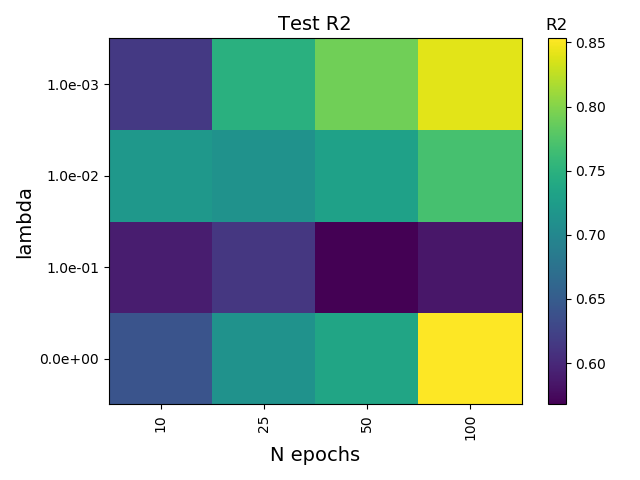
\includegraphics[scale=0.45]{../figures/task_a/test_p15/heatmap_test_p15_lr_constant_Nhyp4434_R2_n_epochs_lambdas.png}
    \caption{$\Nepochs$ vs $\lambda$}
  \end{subfigure}
  \caption{$R^2$ score for different combinations of hyperparameters. All other parameters are set to the best-fit values shown in Table \ref{tab:sgd_best_fit15}.}
  \label{fig:sgd_4}
\end{figure}
Comparing the results more directly with OLS and Ridge, we get Table \ref{tab:sgd_franke_compare}, where we see that our results are not quite as low as OLS and Ridge. However, the amount of parameters we checked was somewhat limited, so a more thorough analysis would have been a good idea. The $R^2$ score for our SGD was around $0.83$, so its not directly bad.
\begin{table}[H]
  \centering
  \caption{Comparison between the test MSE for SGD, OLS, and Ridge for $p=8$ and $p=15$. OLS and Ridge results taken from \cite{Github1}.}
  \label{tab:sgd_franke_compare}
  \begin{tabular}{c|c|c|c}
    \hline\hline
    $p$ & SGD & OLS & Ridge \\\hline
	$8$ & $1.2\cdot10^{-2}$ & $3.3\cdot10^{-3}$ & $3.5\cdot10^{-3}$\\
	$15$& $1.0\cdot10^{-2}$ & $9.7\cdot10^{-3}$ & $3.3\cdot10^{-3}$
    \end{tabular}
\end{table}
To verify our results, we compare to the SGD functionality in the python package Scikit-Learn. Table \ref{tab:sgd_franke_skl} shows the MSE and $R^2$ score for both our code and Scikit-Learn. Confusingly enough, my model seems to outperform the Scikit-Learn method, despite trying to set similar settings, though looking more properly at what it does might reveal some implementation differences not accounted for. Curiously enough, while only the test error is printed here, both my own SGD and SKL gets very similar results for train and test.
\begin{table}[H]
  \centering
  \caption{Comparison between MSE and $R^2$ for our code and Scikit-Learn.}
  \label{tab:sgd_franke_skl}
  \begin{tabular}{c|c|c|c|c}
    \hline\hline
    $p$ & SGD MSE & SKL MSE & SGD $R^2$ & SKL $R^2$\\\hline
	$8$ & $0.012$ & $0.032$ & $0.82$ & $0.53$\\
	$15$& $0.010$ & $0.031$ & $0.84$ & $0.54$
    \end{tabular}
\end{table}
Finally, before moving on to neural networks, we test with a non-constant learning rate. To test this, we set $\Nepochs \in \{10, 25, 50, 75, 100, 200\}$ as well as the different lambdas we tested for earlier. For $t_0 = 1$ and $t_1 = 10$, we get Figure \ref{fig:sgd_5}, which surprisingly shows that the largest regularization is preferred, although the fit itself (with the maximum $R^2$ score at around $0.5$) is not very good. We also see that not just the largest $\Nepochs$ gives the best fit, which makes sense since we scale the learning rate with iterations, and after some point there is no reason to continue iterating.
\begin{figure}[H]
	\centering
	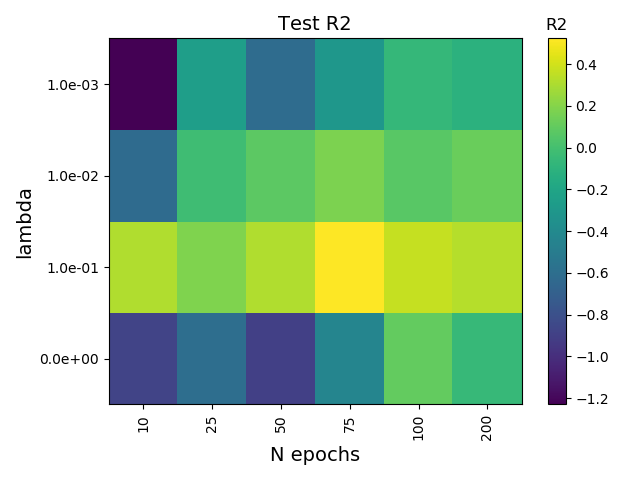
\includegraphics[scale=0.5]{../figures/task_a/non_constant_lr/heatmap_non_constant_lr_lr_optimal_Nhyp6114_R2_n_epochs_lambdas.png}
	\caption{$R^2$ score for number of epochs plotted against regularization $\lambda$ with a learning rate that decreases over time ($t_0 = 1$, $t_1=10$). All other parameters are set to the best-fit values for $p=8$.}
	\label{fig:sgd_5}
\end{figure}

\subsubsection{Feed-forward Neural Network}
Now, it is time to look at the neural network. The design matrix this time is not the polynomial matrix we used for SGD, instead we use the $x$ and $y$ coordinates of the Franke function as our two input predictors. Like with SGD, we have the same hyperparameters from Table \ref{tab:hyper_sgd} as well as the amount of nodes in each hidden layer $\Nhn$, and the amount of hidden layers $\Nhl$. We fit the model with the following parameters
\begin{align*}
	N_{\text{epochs}} &\in \{10, 25, 50, 100\}\\
	\text{batch size} &\in \{1, 5, 10, 50\}\\
	\eta_0 &\in \{0.1, 0.01, 0.001\}\\
	\lambda &\in \{0.0, 0.1, 0.01, 0.001\}\\
	\Nhn &\in \{10, 25, 50\}\\
	\Nhl &= 1
\end{align*}
and a constant learning rate, random weights/bias initialization, and the sigmoid function as the activation function for the hidden layers. It is worth noting that the tests were done with only one hidden layer, as we already had 576 combinations to test, and just adding one more hidden layer would double the amount of testing, which while not the biggest issue with this specific data set, would have caused some problems time wise. This topic is further discussed in Section \ref{sec:za_warudo}. After finding the fit for these parameters we will look at the some combinations of $\Nhn$ and $\Nhl$ directly in order to see if the model prefers higher amounts of hidden layers.
\\\\
Table \ref{tab:nn_franke_best} shows the best fit parameters for the neural net with the combinations specified above. We plot the resulting heatmaps to study how they depend on each other.
\begin{table}[H]
  \centering
  \caption{Best-fit hyperparameters for Franke function using our neural network code. The amount of hidden layers $\Nhl$ had only one combination to test, and mostly added here for completeness.}
  \label{tab:nn_franke_best}
  \begin{tabular}{c|c}
    \hline\hline
    Parameter & Value\\\hline
    $\Nepochs$ &  $100$\\
    batch size &  $50$\\
    $\eta_0$ & $0.1$ \\
    $\lambda$ & $0.001$\\
    $\Nhn$ & $25$\\
    $\Nhl$ & $1$
    \end{tabular}
\end{table}
Figure \ref{fig:nn_1} shows the $R^2$ heatmaps for 5 combinations of hyperparameters plotted against each other. Panel (a) shows the same behavior we saw for SGD, with the lowest amounts of epochs and learning rate does not have time to converge. Panel (b) shows is a bit interesting though, as unlike SGD, it seems to vastly prefer larger minibatches. The batch size will be discussed a bit more later when comparing to Scikit-Learn. Panel (c) shows the that the largest regularization performs the worst, like with SGD. The preferred model however is the smallest $\lambda$ combined with the highest $\Nepochs$. Panel (d) shows that few combinations are "good", however the scale on the $z$ axis starts at roughly $R^2 = 0.74$, so the differences aren't too large. Panel (e) shows that the largest learning rate gives the best results regardless of $\Nhn$.
\begin{figure}[H]
  \centering
  \begin{subfigure}{0.49\textwidth}
    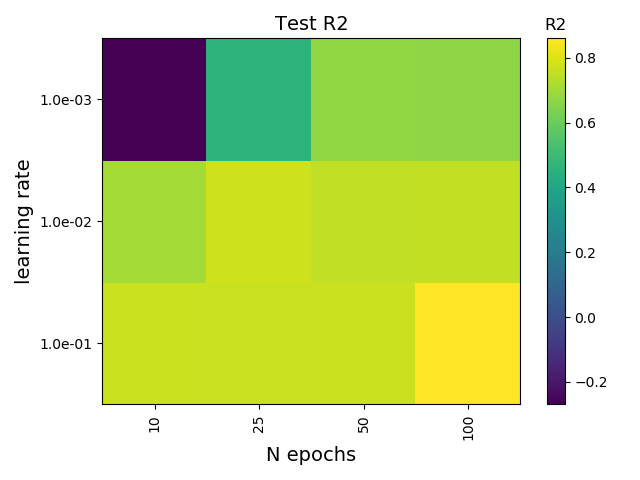
\includegraphics[scale=0.45]{../figures/task_b/test/heatmap_test_lr_constant_Nhyp443431_R2_n_epochs_eta0.png}
    \caption{$\Nepochs$ vs learning rate}
  \end{subfigure}
  \begin{subfigure}{0.49\textwidth}
    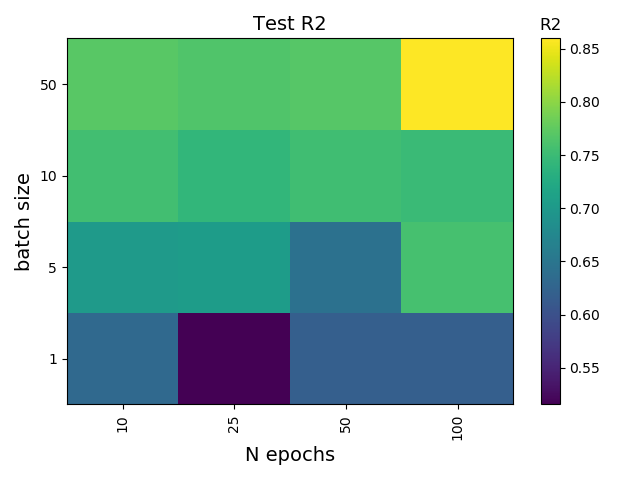
\includegraphics[scale=0.45]{../figures/task_b/test/heatmap_test_lr_constant_Nhyp443431_R2_n_epochs_bsize.png}
    \caption{$\Nepochs$ vs batch size}
  \end{subfigure}\\
  \begin{subfigure}{0.49\textwidth}
    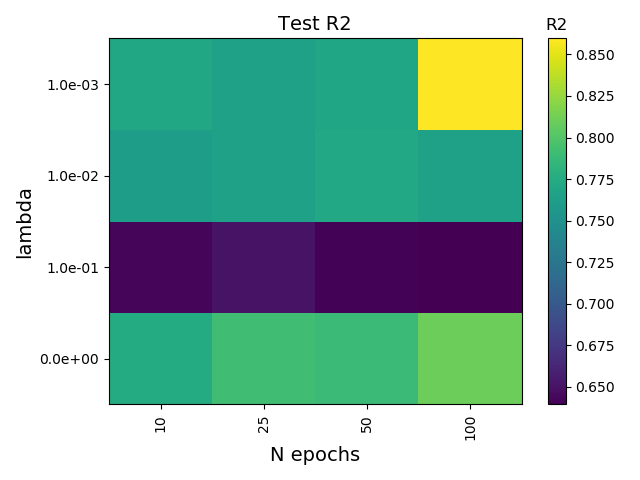
\includegraphics[scale=0.45]{../figures/task_b/test/heatmap_test_lr_constant_Nhyp443431_R2_n_epochs_lambdas.png}
    \caption{$\Nepochs$ vs $\lambda$}
  \end{subfigure}
  \begin{subfigure}{0.49\textwidth}
    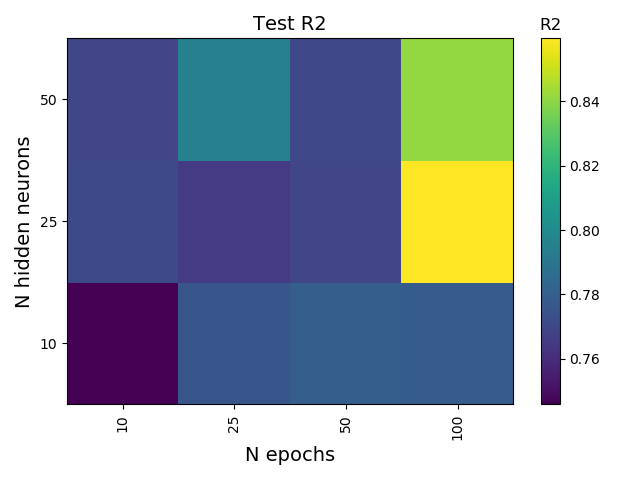
\includegraphics[scale=0.45]{../figures/task_b/test/heatmap_test_lr_constant_Nhyp443431_R2_n_epochs_nhn.png}
    \caption{$\Nepochs$ vs $\Nhn$}
  \end{subfigure}\\
    \begin{subfigure}{0.49\textwidth}
    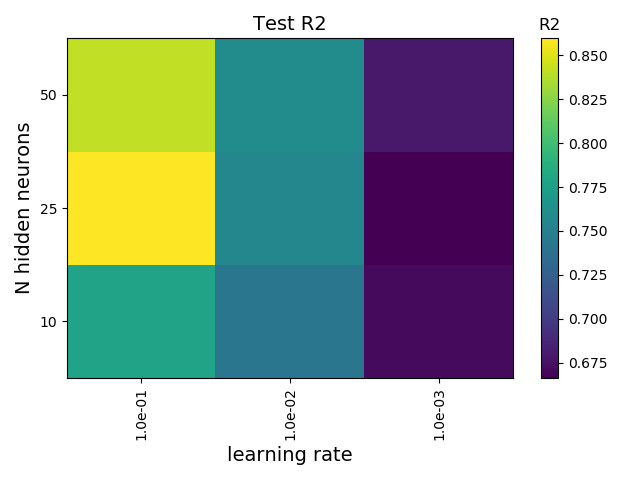
\includegraphics[scale=0.45]{../figures/task_b/test/heatmap_test_lr_constant_Nhyp443431_R2_eta0_nhn.png}
    \caption{Learning rate vs $\Nhn$}
  \end{subfigure}
  \caption{$R^2$ score for different combinations of hyperparameters. All other parameters are set to the best-fit values shown in Table \ref{tab:nn_franke_best}.}
  \label{fig:nn_1}
\end{figure}
Finally, Table \ref{tab:nn_franke_results} shows the MSE (and $R^2$ for NN/SGD) score for NN, SGD, OLS and Ridge. We see that our neural network outperforms the SGD by a factor of 2, though is still not quite as good as OLS or Ridge. That said, we did not take the amount of hidden layers into consideration, and it is worth checking how changing the activation function affects the results. The final $R^2$ score for our neural net is $0.93$ though, which is a really good fit.
\begin{table}[H]
  \centering
	\caption{Comparison between MSE scores for NN, SGD, OLS and Ridge. The $R^2$ score is added for NN and SGD, however the same results for OLS and Ridge are not available without going back to the code used in \cite{Github1}.}
  \label{tab:nn_franke_results}
  \begin{tabular}{c|c|c}
    \hline\hline
    Method & MSE & $R^2$\\\hline
	NN & $5.0\cdot10^{-3}$ & $0.93$ \\
	SGD & $1.0\cdot10^{-2}$& $0.84$ \\
	OLS & $3.3\cdot10^{-3}$& -\\
	Ridge & $3.3\cdot10^{-3}$& -
    \end{tabular}
\end{table}

\subsubsection*{Testing the amount of hidden layers}
Since our best-fit found previously didn't take the amount of hidden layers into consideration, we perform a test where all the other parameters except the amount of hidden layers and nodes per hidden layer is kept at the best-fit parameters from Table \ref{tab:nn_franke_best}. We test the following combinations
\begin{align*}
	\Nhn &\in \{10, 25, 50\}\\
	\Nhl &\in \{1, 2, 3, 4\}
\end{align*}
Figure \ref{fig:nn_params_franke} shows the $R^2$ score heatmap for $\Nhn$ plotted against $\Nhl$. We see that the trend is towards a higher amount of total nodes ($\Nhl\cdot\Nhn$), however the best fit is for 4 hidden layers and 25 nodes per layer. All of them however give a fit of $R^2 > 0.8$, so none of them are bad.
\begin{figure}[H]
	\centering
	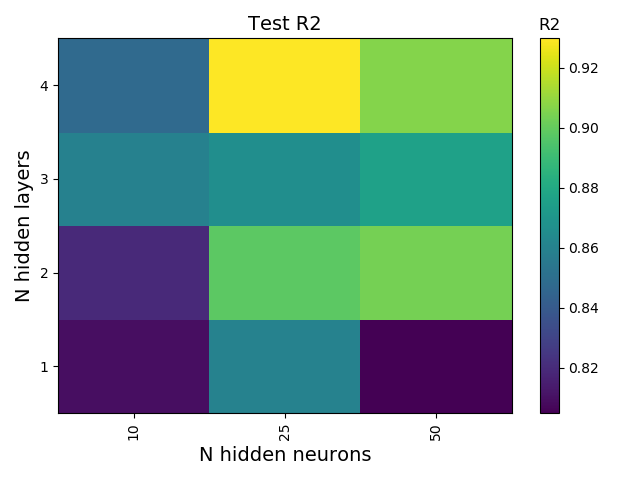
\includegraphics[scale=0.5]{../figures/task_b/nn_parameters/heatmap_nn_parameters_lr_constant_Nhyp111134_R2_nhn_nhl.png}
	\caption{$R^2$ score for number of hidden layers vs number of nodes per hidden layer. All other parameters are set to the best-fit values.}
	\label{fig:nn_params_franke}
\end{figure}


\subsubsection*{Testing different activation functions}
We test different activation functions for the hidden layers in order to see how the results depend on it. The results of this is shown in Table \ref{tab:franke_actfunc}, with the Scikit-Learn results added for reference. Interestingly enough, the using the sigmoid/logistic function gives us the worst fit of them all. The tanh-function almost halves the MSE with the sigmoid function, and both ReLu's are almost 1/5th of the sigmoid function. Using the leaky ReLu we end up with an $R^2$ score that is almost 0.9, which is extremely good. Scikit-learn however is a bit better then our sigmoid results, despite using the same parameters.
\begin{table}[H]
  \centering
  \caption{Comparison between the train/test MSE and $R^2$ scores for different activation functions. The hyperparameters are $\Nepochs=50$, batch size$=1$, $\eta_0=0.1$, $\lambda=0$, and one hidden layer with 25 nodes. For reference, the Scikit-Learn value found using the logistic function as $\sigma(z)$ is added to the bottom.}
  \label{tab:franke_actfunc}
  \begin{tabular}{c|c|c|c|c}
    \hline\hline
    $\sigma(z)$ & Train MSE & Test MSE & Train $R^2$ & Test $R^2$\\\hline
	sigmoid & $0.027$ & $0.030$ & $0.586$ & $0.566$\\
	ReLu & $0.006$ & $0.007$ & $0.904$ & $0.888$\\
	leaky ReLu & $0.006$ & $0.007$ & $0.909$ & $0.893$\\
	tanh & $0.014$ & $0.015$ & $0.784$ & $0.768$\\\hline
	SKL & $0.021$ & $0.023$ & $0.685$ & $0.653$\\\hline
    \end{tabular}
\end{table}

\subsubsection*{Batch sizes and comparison with Scikit-Learn}
As noted earlier, Figure \ref{fig:nn_1} panel (b) showed that the system highly prefers larger minibatches, differing somewhat from how SGD behaved. In order to test this we will compare our results with Scikit-Learn, using mostly the same parameter choices as our best fit. We plot the loss function directly for each epoch, but for some reason adding regularization to the mix seems to cause some scaling difference with how it is added to the loss function, so we disregard it here.
\\\\
Figure \ref{fig:nn_franke_skl} shows the loss curve comparison between our code and Scikit-Learn for batch sizes 1 and 50. We see that for batch size $=1$, our own code follows the SKL curve very closely, with some start difference that may stem from SKL using Glorot initialization \cite{glorot} for their weights and bias. Also, SKL stops before reaching the maximum number of epochs, which we failed to deactivate. For batch size 50 however, our results are extremely different, yielding much better results than SKL. This could be due to how the minibatches are made and drawn for each iteration, but after looking at the code for MLPRegressor I am not sure how much of a difference there is.
\begin{figure}[H]
  \centering
  \begin{subfigure}{0.49\textwidth}
    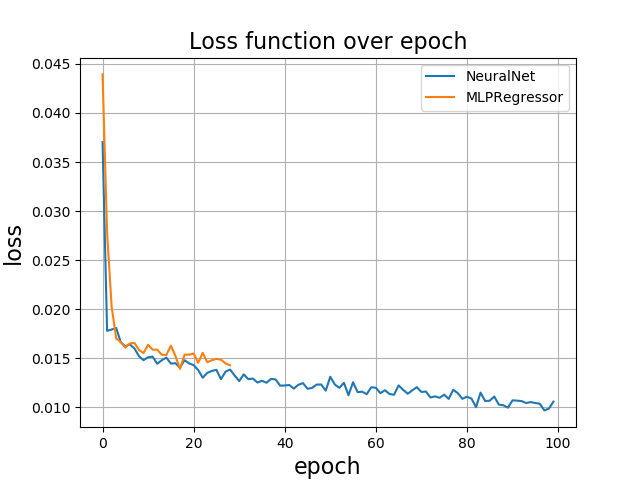
\includegraphics[scale=0.45]{../figures/task_b/minibatch1/loss.png}
    \caption{Batch size $=1$}
  \end{subfigure}
  \begin{subfigure}{0.49\textwidth}
    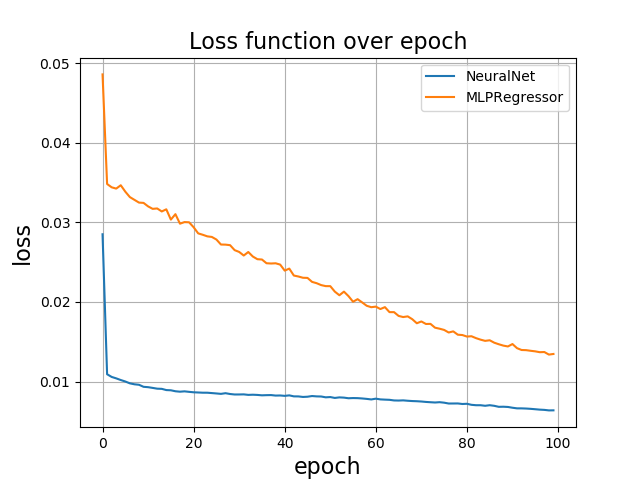
\includegraphics[scale=0.45]{../figures/task_b/minibatch50/loss.png}
    \caption{Batch size $=50$}
  \end{subfigure}
  \caption{Loss curve plotted against epoch for both our code and Scikit-Learn's MLPRegressor. Left panel shows batch size $=1$, while right panel shows batch size $=50$. Parameters are the best-fit, except that $\lambda = 0$.}
  \label{fig:nn_franke_skl}
\end{figure}
The same results can be seen in Table \ref{tab:nn_franke_skl}, where we see that both the MSE and $R^2$ score is better for both of the batch sizes.
\begin{table}[H]
  \centering
  \caption{Comparison between MSE and $R^2$ for our code and Scikit-Learn, with different batch sizes. Parameters are the best-fit, except that $\lambda = 0$.}
  \label{tab:nn_franke_skl}
  \begin{tabular}{c|c|c|c|c}
    \hline\hline
    batch size & NN MSE & SKL MSE & NN $R^2$ & SKL $R^2$\\\hline
	1 & $0.013$ & $0.037$ & $0.803$ & $0.442$\\
	50& $0.011$ & $0.030$ & $0.838$ & $0.553$
    \end{tabular}
\end{table}
\subsubsection*{Weights and bias initialization}
We briefly look at how the results depend on initialization. Figure \ref{fig:nn_franke_skl_init} shows the loss curve for our code using either random or Glorot initialization. We see that our results are better when using random initialization , and more in line with what MLPRegressor gets (until it stops) despite it using Glorot initialization.
\begin{figure}[H]
  \centering
  \begin{subfigure}{0.49\textwidth}
    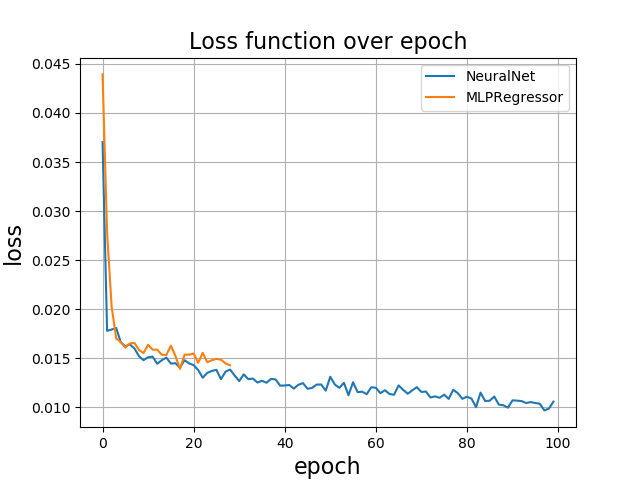
\includegraphics[scale=0.45]{../figures/task_b/minibatch1/loss.png}
    \caption{Random initialization}
  \end{subfigure}
  \begin{subfigure}{0.49\textwidth}
    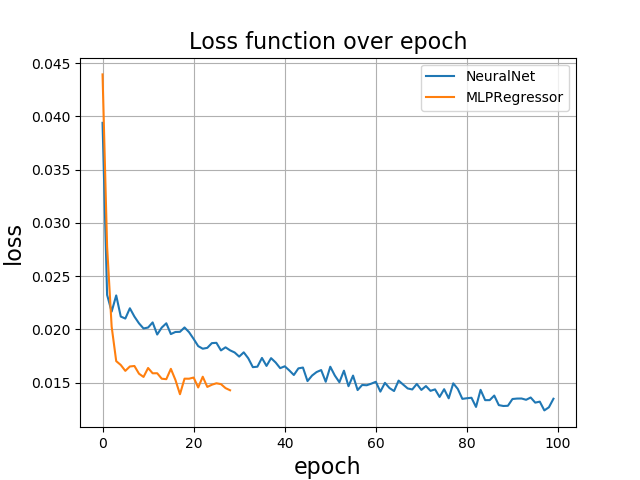
\includegraphics[scale=0.45]{../figures/task_b/minibatch1_glorot/loss.png}
    \caption{Glorot initialization}
  \end{subfigure}
  \caption{Loss curve plotted against epoch for both our code and Scikit-Learn's MLPRegressor, with different weights/bias initialization scheme. Parameters are the best-fit, except that $\lambda = 0$. Both of the SKL plots use Glorot initialization.}
  \label{fig:nn_franke_skl_init}
\end{figure}

\subsubsection*{Non-constant learning rate}
Lastly, we take a look at using a scaling learning rate instead of constant. We use the best fit settings with batch size set to 1 and $\lambda = 0$. Figure \ref{fig:nn_franke_skl_lr} shows the loss curve with learning rate set to the one discussed earlier, with $t_0 = 1$ and $t_1 = 10$. We see that until the point that SKL stops, our own code follows, which is similar to what we saw with a constant learning rate. However afterwards, the loss barely changes, which makes sense as the learning rate gets vanishingly small as the iteration count increases, so stopping around the point where SKL stops seems to make sense in that case (despite SKL using a constant learning rate, so not sure why it ends up stopping there). This corresponds to an $R^2$ score of about $0.66$, which is not nearly as good as we got for the constant learning rate.
\begin{figure}[H]
  \centering
  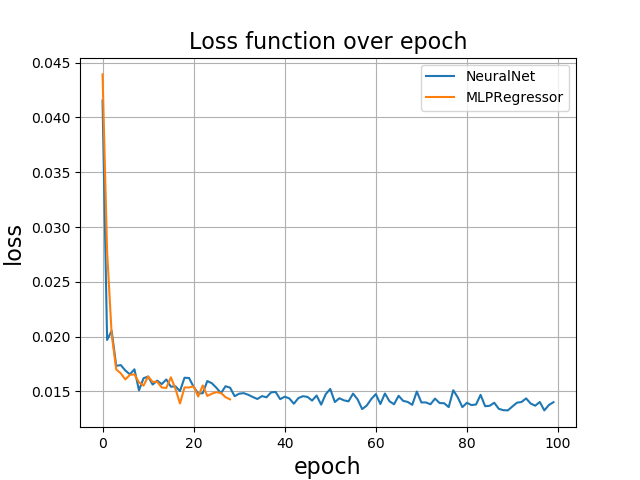
\includegraphics[scale=0.45]{../figures/task_b/minibatch1_optimal/loss.png}
  \caption{Loss curve plotted against epoch for both our code and Scikit-Learn's MLPRegressor, with non-constant. Parameters are the best-fit, with batch size $=1$ and $\lambda = 0$}
  \label{fig:nn_franke_skl_lr}
\end{figure}

\subsection{MNIST data set}
In this section we will be looking at the results from analysing the reduced MNIST data set described in Chapter \ref{chap:data_sets}. The design matrix we use for both the NN and SGD results will be all the images, with each pixels as one predictor. This gives us an $1797\times64$ design matrix.

\subsubsection{Classification with Neural Network}
Using the same neural network code as for the Franke function, we have the same hyperparameters to adjust. The activation function for the hidden layer is the sigmoid function like with the regression case, but the output activation function is set to the softmax function, and the loss function as cross-entropy. We fit our model using the following parameter sets (the same as for the Franke function)
\begin{align*}
	N_{\text{epochs}} &\in \{10, 25, 50, 100\}\\
	\text{batch size} &\in \{1, 5, 10, 50\}\\
	\eta_0 &\in \{0.1, 0.01, 0.001\}\\
	\lambda &\in \{0.0, 0.1, 0.01, 0.001\}\\
	\Nhn &\in \{10, 25, 50\}\\
	\Nhl &= 1
\end{align*}
Table \ref{tab:nn_mnist_best} shows the best fit parameters for the neural net with the combinations specified above. Oddly, for some reason based on the parameters it seems like the neural net converges extremely fast given the number of epochs and size of the hidden layer. 
\begin{table}[H]
  \centering
  \caption{Best-fit hyperparameters for the MNIST data set using our neural network code. The amount of hidden layers $\Nhl$ had only one combination to test, and mostly added here for completeness.}
  \label{tab:nn_mnist_best}
  \begin{tabular}{c|c}
    \hline\hline
    Parameter & Value\\\hline
    $\Nepochs$ &  $10$\\
    batch size &  $5$\\
    $\eta_0$ & $0.1$ \\
    $\lambda$ & $0.01$\\
    $\Nhn$ & $10$\\
    $\Nhl$ & $1$
    \end{tabular}
\end{table}
Table \ref{tab:nn_mnist_accuracy} shows the accuracy for our NN-code compared to Scikit-Learn using our best-fit parameters. Our NN-code performs extremely well, being even better than Scikit-Learn, with a test accuracy of almost 95\%. It is worth noting that SKL complains complains that there is not enought iterations to converge. Setting the max iterations higher allowed changes the test accuracy to 90\%, which is still not as high as our own code.
\begin{table}[H]
  \centering
  \caption{Comparison between the accuracy score for our NN code and Scikit-Learn using best-fit parameters.}
  \label{tab:nn_mnist_accuracy}
  \begin{tabular}{c|c|c}
    \hline\hline
    Method & Train accuracy & Test accuracy\\\hline
	NN & $0.987$ & $0.949$\\
	SKL & $0.908$ & $0.850$
    \end{tabular}
\end{table}
We then plot the resulting heatmaps to study how they depend on each other. Figure \ref{fig:nn__mnist1} shows the accuracy heatmaps for different combinations of hyperparameters. In panel (a) we see the same relation between $\Nepochs$ and learning rate that we saw earlier in both SGD and NN for the Franke function. Panel (b) shows the opposite dependency upon batch size, however looking at the $z$-axis, the difference is only around $3$\% in the accuracy. 
\\\\
Panel (c) shows that the two lowest $\lambda$ values are preferred, though no regularization performs the worst. The difference is only around 5\% though. Panel (d) shows surprisingly shows that the highest $\Nepochs$ and $\Nhn$ yields the best accuracy, and the worst for the lowest combination. The best fit-parameters however was with he lowest parameter combination, so it shows how interconnected the parameters are, though the difference in that plot is only 3\%. Finally, panel (e) shows similar results to earlier.
\begin{figure}[H]
  \centering
  \begin{subfigure}{0.49\textwidth}
    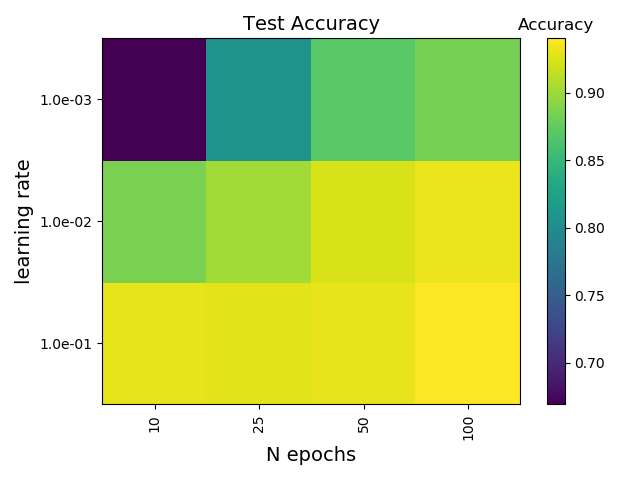
\includegraphics[scale=0.45]{../figures/task_d/test/heatmap_test_lr_constant_Nhyp443431_Accuracy_n_epochs_eta0.png}
    \caption{$\Nepochs$ vs learning rate}
  \end{subfigure}
  \begin{subfigure}{0.49\textwidth}
    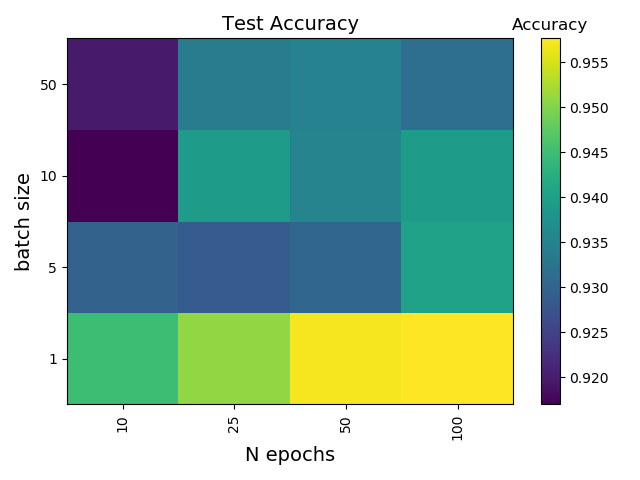
\includegraphics[scale=0.45]{../figures/task_d/test/heatmap_test_lr_constant_Nhyp443431_Accuracy_n_epochs_bsize.png}
    \caption{$\Nepochs$ vs batch size}
  \end{subfigure}\\
  \begin{subfigure}{0.49\textwidth}
    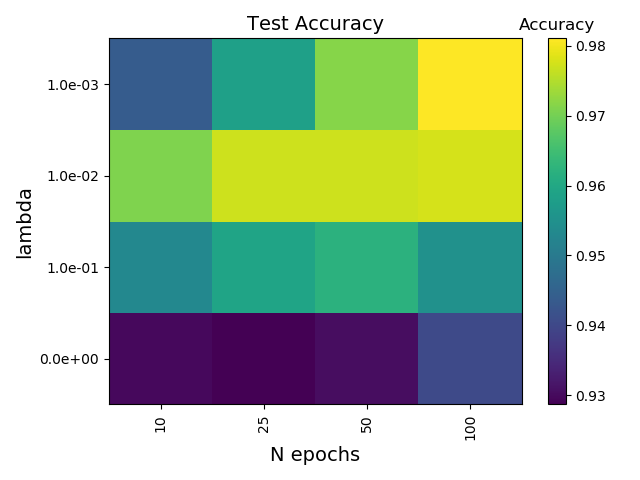
\includegraphics[scale=0.45]{../figures/task_d/test/heatmap_test_lr_constant_Nhyp443431_Accuracy_n_epochs_lambdas.png}
    \caption{$\Nepochs$ vs $\lambda$}
  \end{subfigure}
  \begin{subfigure}{0.49\textwidth}
    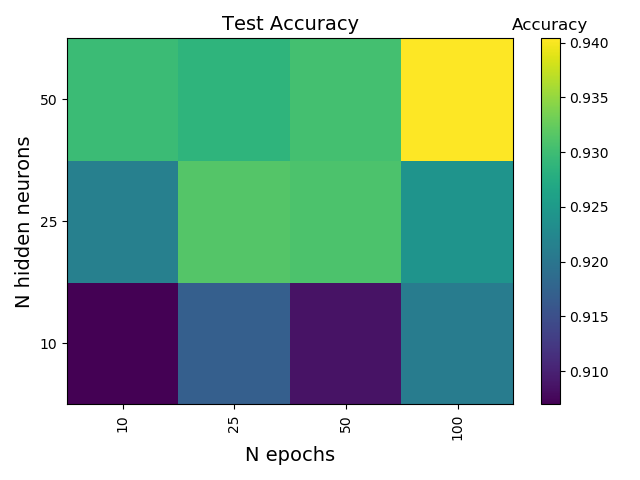
\includegraphics[scale=0.45]{../figures/task_d/test/heatmap_test_lr_constant_Nhyp443431_Accuracy_n_epochs_nhn.png}
    \caption{$\Nepochs$ vs $\Nhn$}
  \end{subfigure}\\
    \begin{subfigure}{0.49\textwidth}
    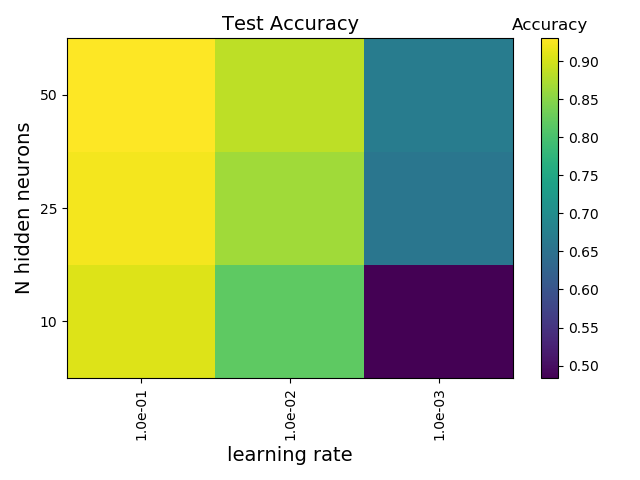
\includegraphics[scale=0.45]{../figures/task_d/test/heatmap_test_lr_constant_Nhyp443431_Accuracy_eta0_nhn.png}
    \caption{Learning rate vs $\Nhn$}
  \end{subfigure}
  \caption{Accuracy score for different combinations of hyperparameters. All other parameters are set to the best-fit values shown in Table \ref{tab:nn_mnist_best}.}
  \label{fig:nn__mnist1}
\end{figure}
\subsubsection*{Testing the amount of hidden layers}
We test what happens when we let only the amount of nodes and amount of hidden layers to vary, testing the following combinations. All other parameters are set to the best-fit.
\begin{align*}
	\Nhn &\in \{10, 25, 50\}\\
	\Nhl &\in \{1, 2, 3, 4\}
\end{align*}
Figure \ref{fig:nn_params_mnist} shows the accuracy score heatmap for $\Nhn$ plotted against $\Nhl$. We see that for each $\Nhn$, the accuracy decreases the more layers are added, contrasting how it worked in the regression case. This does however mean that the best-fit $\Nhl$ would have been $1$ had we included more than one value.
\begin{figure}[H]
	\centering
	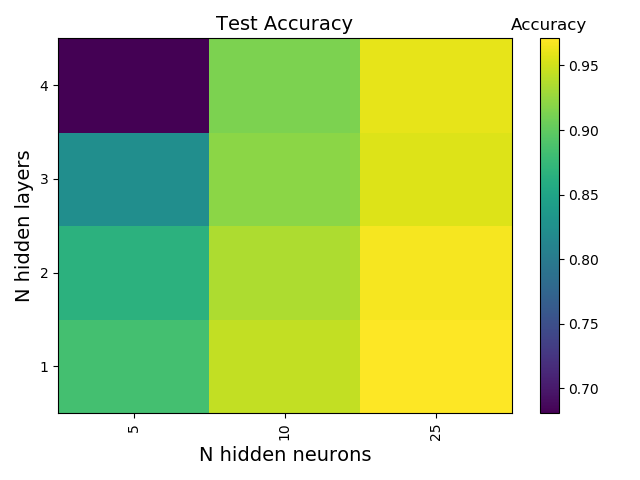
\includegraphics[scale=0.5]{../figures/task_d/nn_parameters/heatmap_nn_parameters_lr_constant_Nhyp111134_Accuracy_nhn_nhl.png}
	\caption{Accuracy score for number of hidden layers vs number of nodes per hidden layer. All other parameters are set to the best-fit values.}
	\label{fig:nn_params_mnist}
\end{figure}


\subsubsection*{Testing different activation functions}
We test different activation functions for the hidden layers in order to see how the results depend on it. The results of this is shown in Table \ref{tab:mnist_actfunc}. Both of the ReLu functions end up with a divide by zero error, causing the results to be horrible. Both the logistic function (sigmoid) and tanh gives similar and good results, with the logistic function being slightly better.
\begin{table}[H]
  \centering
  \caption{Comparison between the train/test accuracy score for different activation functions. The hyperparameters are the best-fit found earlier.}
  \label{tab:mnist_actfunc}
  \begin{tabular}{c|c|c}
    \hline\hline
    $\sigma(z)$ & Train accuracy & Test accuracy\\\hline
	sigmoid & $0.987$ & $0.949$ \\
	ReLu & $0.099$ & $0.099$ \\
	leaky ReLu & $0.099$ & $0.099$ \\
	tanh & $0.966$ & $0.926$ \\
    \end{tabular}
\end{table}

\subsubsection{Logistic regression}
Finally, we want to use our SGD code to fit the MNIST data set. We test the following combinations of hyperparameters, setting the learning rate to constant.
\begin{align*}
	N_{\text{epochs}} &\in \{10, 25, 50, 100\}\\
	\text{batch size} &\in \{1, 5, 10, 50\}\\
	\eta_0 &\in \{0.1, 0.01, 0.001\}\\
	\lambda &\in \{0.0, 0.1, 0.01, 0.001\}
\end{align*}
Table \ref{tab:sgd_best_fit_mnist} shows the best-fit parameters for this data set and set of hyperparameters. Unlike the NN, the model might take longer to converge as the highest $\Nepochs$ is chosen, though the learning rate is also the lowest. The regularization factor is also the largest one.
\begin{table}[H]
  \centering
  \caption{Best-fit hyperparameters for the MNIST data set using SGD for logistic regression.}
  \label{tab:sgd_best_fit_mnist}
  \begin{tabular}{c|c}
    \hline\hline
    Parameter & Value\\\hline
    $\Nepochs$ &  $100$\\
    batch size &  $1$\\
    $\eta_0$ & $0.001$ \\
    $\lambda$ & $0.1$
    \end{tabular}
\end{table}
Table \ref{tab:sgd_mnist_accuracy} shows the accuracy for our SGD-code compared to Scikit-Learn using our best-fit parameters. Like with the neural net, our SGD code performs extremely well, ending up with a test accuracy of 96\%, even better than the NN. SKL is also very close, though some of that is due to having enough time to converge unlike the problems it had in the NN case.
\begin{table}[H]
  \centering
  \caption{Comparison between the accuracy score for our SGD code and Scikit-Learn using best-fit parameters.}
  \label{tab:sgd_mnist_accuracy}
  \begin{tabular}{c|c|c}
    \hline\hline
    Method & Train accuracy & Test accuracy\\\hline
	NN & $0.986$ & $0.960$\\
	SKL & $0.971$ & $0.956$
    \end{tabular}
\end{table}

\subsubsection*{Hyperparameter heatmaps}
Figure \ref{fig:sgd_mnist1} shows the Accuracy heatmaps for some combinations of hyperparameters. In panel (a) we see that for all possible $\Nepochs$, the results get better as the learning rate is decreased. Panel (b) shows that the smallest batch sizes gives the best results, which behaves roughly as it did for NN with classification. Panel (c) shows that the best regularization is the largest $\lambda$, however the $z$-axis also shows that the difference in percentage isn't that massive.
\begin{figure}[H]
  \centering
  \begin{subfigure}{0.49\textwidth}
    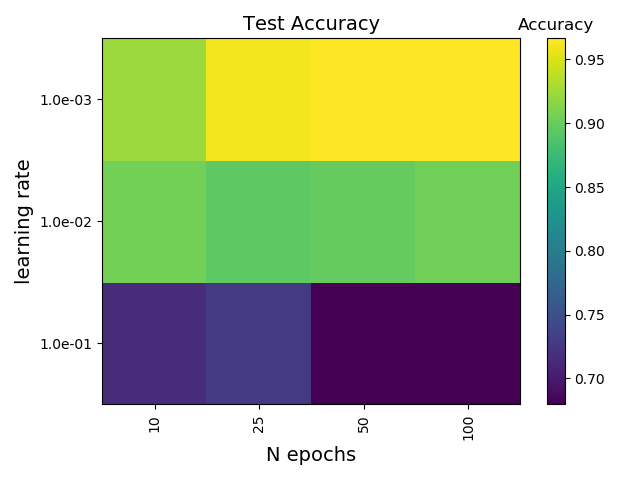
\includegraphics[scale=0.45]{../figures/task_e/test/heatmap_test_lr_constant_Nhyp4434_Accuracy_n_epochs_eta0.png}
    \caption{$\Nepochs$ vs learning rate}
  \end{subfigure}
  \begin{subfigure}{0.49\textwidth}
    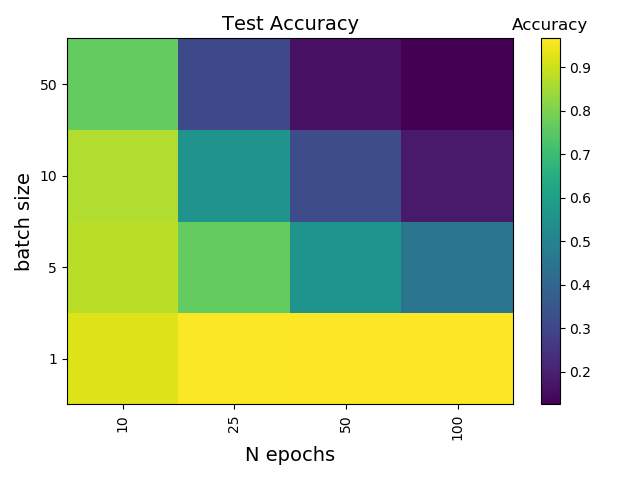
\includegraphics[scale=0.45]{../figures/task_e/test/heatmap_test_lr_constant_Nhyp4434_Accuracy_n_epochs_bsize.png}
    \caption{$\Nepochs$ vs batch size}
  \end{subfigure}\\
  \begin{subfigure}{0.49\textwidth}
    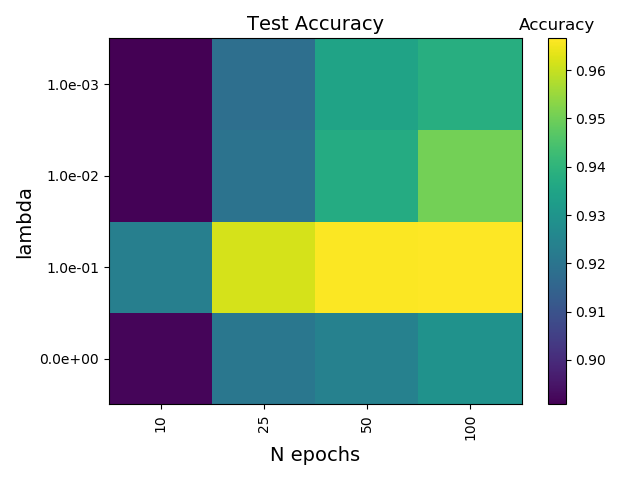
\includegraphics[scale=0.45]{../figures/task_e/test/heatmap_test_lr_constant_Nhyp4434_Accuracy_n_epochs_lambdas.png}
    \caption{$\Nepochs$ vs $\lambda$}
  \end{subfigure}
  \caption{Accuracy score for different combinations of hyperparameters. All other parameters are set to the best-fit values shown in Table \ref{tab:sgd_best_fit_mnist}.}
  \label{fig:sgd_mnist1}
\end{figure}

\subsubsection*{Non-constant learning rate}
Finally, we test with a non-constant learning rate. We set $\Nepochs \in \{10, 25, 50, 75, 100, 200\}$ as well as the different lambdas we tested for earlier. For $t_0 = 1$ and $t_1 = 10$, we get Figure \ref{fig:sgd_mnist2}. We see that in this case, the largest $\lambda$ value is still preferred, similar to when we did the same for the Franke function SGD model (though then, with a constant learning rate, the preferred $\lambda$ was either the lowest or zero). The accuracy is best for $\Nepochs= 100$, and decreases slightly going above that. Testing other values of $t_0$ and $t_1$ would have been a good idea.
\begin{figure}[H]
	\centering
	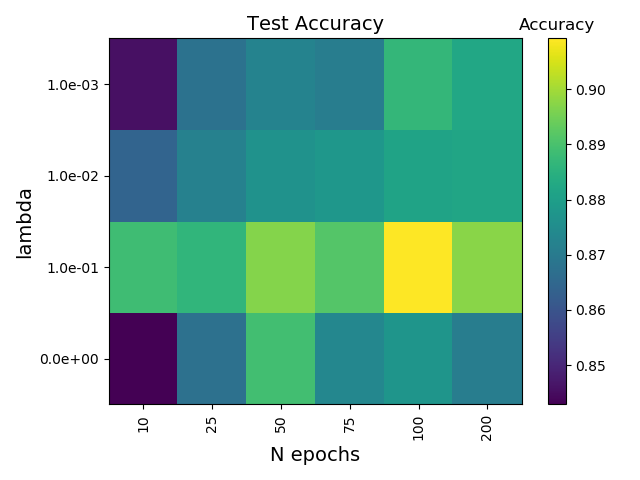
\includegraphics[scale=0.5]{../figures/task_e/non_constant_lr/heatmap_non_constant_lr_lr_optimal_Nhyp6114_Accuracy_n_epochs_lambdas.png}
	\caption{Accuracy score for number of epochs plotted against regularization $\lambda$ with a learning rate that decreases over time ($t_0 = 1$, $t_1=10$). All other parameters are set to the best-fit values.}
	\label{fig:sgd_mnist2}
\end{figure}


\subsection{Training time} \label{sec:za_warudo}
One of the big problems with methods like the stochastic gradient descent and neural networks is the high amount of hyperparameters to tweak. In this project, we used grid-search in order to try to find the optimal values for all our hyperparameters. This is a method that lends itself very well to parallelization as each parameter combination is independent of each other, though you have to go through a lot of combinations. Sadly, there was no time to implement parallelization for this project.
\\\\
For the neural net results in this project, we looked at a set of 576 combinations when trying to find the optimal fit. For the Franke function, this did not take too long, but for the classification problem, this took 15.5 hours to complete. Which is why we ended up avoiding to run with more than one hidden layer in the main fit procedure, as a time estimate was made when deciding upon which parameters to try.
\\\\
Imagine then if we were to use the full MNIST data set instead of the reduced one we used here, we would end up with a design matrix with almost 55 million elements
compared to the 115 thousand elements we had in this report. At the very least, having a functional stopping criteria for the gradients would be beneficial. It also shows the importance of better methods for searching for hyperparameters (if you even have time to fit the models more than once), as well as doing research about what others have found. 

%%%%%%%%%%%%%%%%%%%%%%%%%%%%%%%%%%%%%%%%%%%%%%%%%%%%%%%%%%%%%%%%%%%%%%%%%%%%%%%%%%%%%%%%%%
%%%%%%%%%%%%%%%%%%%%%%%%%%%%%%%%%%%%%%%%%%%%%%%%%%%%%%%%%%%%%%%%%%%%%%%%%%%%%%%%%%%%%%%%%%
\section{Conclusion} \label{chap:conclusion}
In this project, we set out to investigate how stochastic gradient descent and feed-forward neural networks work on both regression and classification problems. We used cross-validation in order to assess which of the hyperparameter combinations gave the best fit.
\\\\
For the Franke function, we found that both SGD and FFNN performed worse than OLS and Ridge, though the neural net got much closer, with an $R^2$ score of $0.93$, while SGD got $0.84$, none of which are bad. For both, we found that the largest number of epochs $\Nepochs = 100$ and the largest learning rate $\eta=0.1$ gave the best results. SGD preferred a batch size of 5, with no regularization for $p=8$, and $\lambda=0.001$ at $p=15$, showing similar behavior with how OLS and Ridge performed for those polynomial degrees. The neural net yielded much better results as the batch size is increased. Based on tests, it seems that using either one of the ReLu family activation functions would have improved the results.
\\\\
For the classification case, where we studied a reduced version of the MNIST data set, both the SGD and Neural net performed exceedingly well, outperforming the equivalent Scikit-Learn implementation. The SGD implementation gave an accuracy of 96\%, which starts to approach what you would expect from human accuracy. SKL was within a percent point away from it. The NN code yielded an accuracy of 95\%, but doing so with only 10 epochs and 10 nodes in the singular hidden layer. 
%%%%%%%%%%%%%%%%%%%%%%%%%%%%%%%%%%%%%%%%%%%%%%%%%%%%%%%%%%%%%%%%%%%%%%%%%%%%%%%%%%%%%%%%%%
%%%%%%%%%%%%%%%%%%%%%%%%%%%%%%%%%%%%%%%%%%%%%%%%%%%%%%%%%%%%%%%%%%%%%%%%%%%%%%%%%%%%%%%%%%
\bibliography{references}
%%%%%%%%%%%%%%%%%%%%%%%%%%%%%%%%%%%%%%%%%%%%%%%%%%%%%%%%%%%%%%%%%%%%%%%%%%%%%%%%%%%%%%%%%%
%%%%%%%%%%%%%%%%%%%%%%%%%%%%%%%%%%%%%%%%%%%%%%%%%%%%%%%%%%%%%%%%%%%%%%%%%%%%%%%%%%%%%%%%%%


\end{document}